\documentclass{beamer}
\usepackage[ngerman]{babel}
\usepackage[utf8]{inputenc}     % UTF8-Encoding
\usepackage[T1]{fontenc}        % T1-Schriftkodierung
\usepackage{lmodern}            % Ersetzung der CM-Schrift
\usepackage{listingsutf8}       % Listings (mit UTF8)
\usepackage{array}              % neue Spaltenmodi
\usepackage{textcomp}           % spezielle Zeichen im Text
\usepackage[ngerman]{varioref}  % variable Verweise
\usepackage{scrextend}          % für Labeling
\usepackage{booktabs}           % spezielle Linien in Tabellen
\usepackage{graphicx}

\makeatletter

\usetheme{Szeged}
\usecolortheme{whale}
\titlegraphic{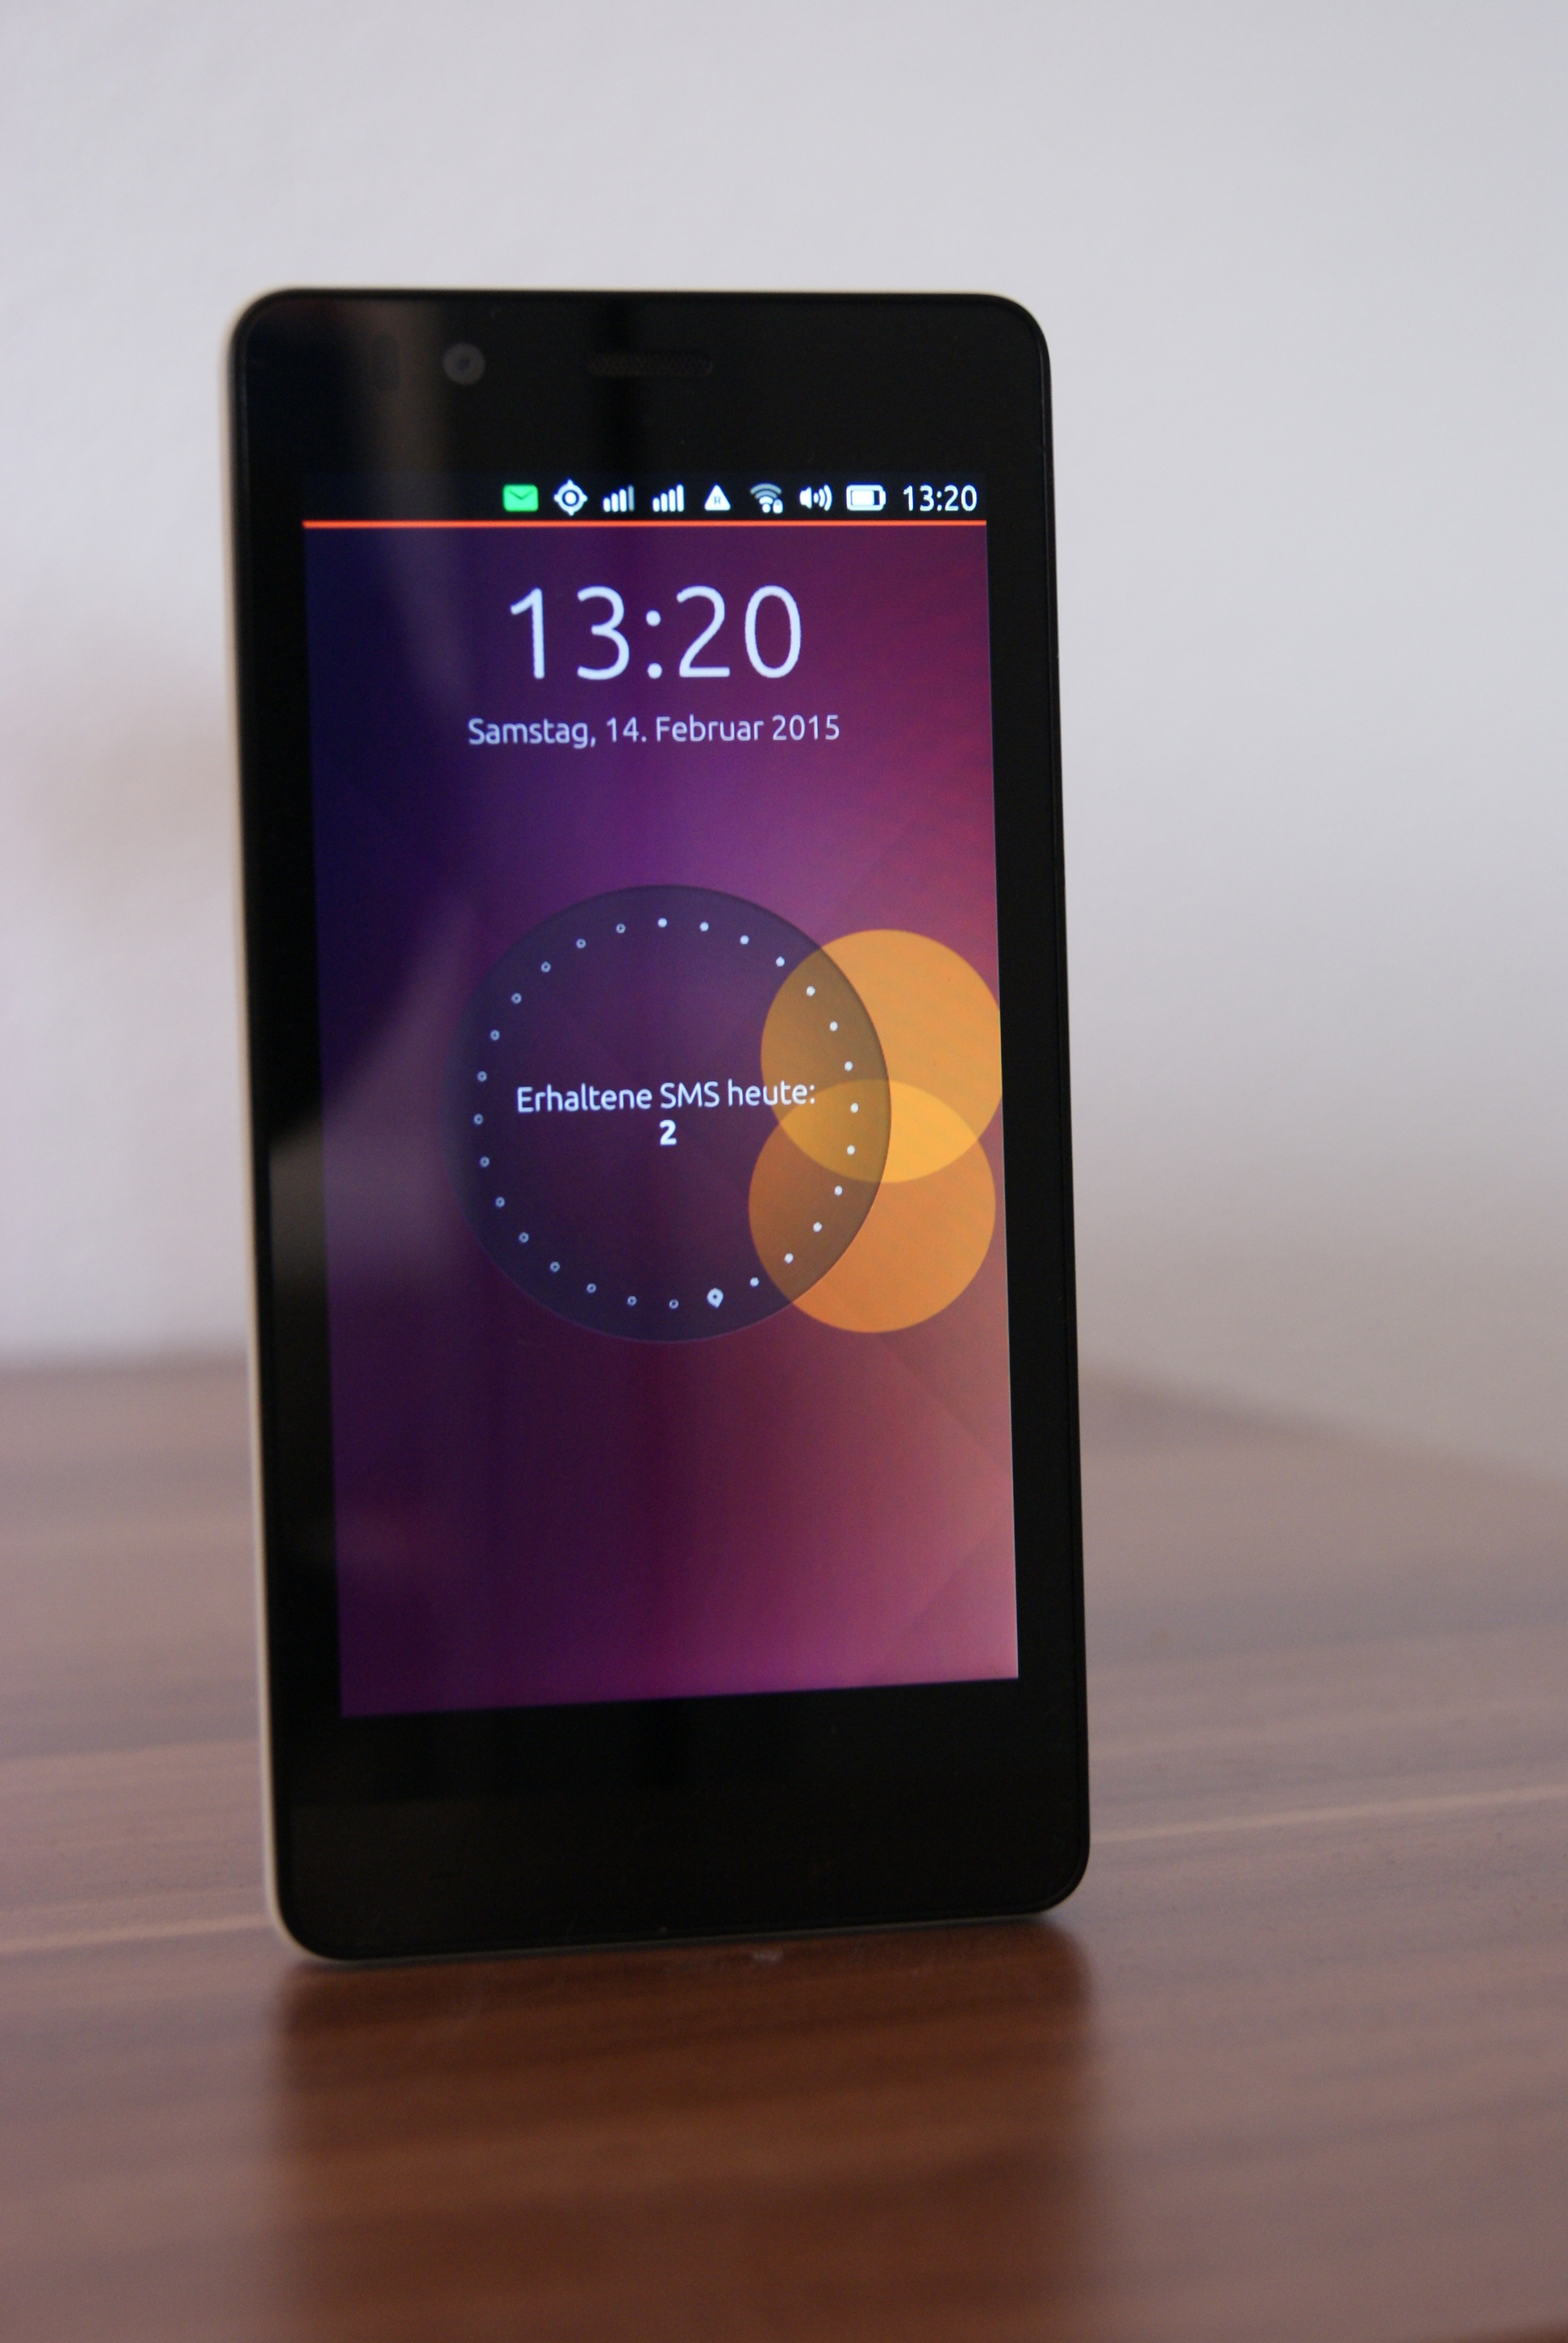
\includegraphics[width=0.2\linewidth]{images/ubuntuphone}}
\title{Ubuntu Phone}
\author{Sujeevan Vijayakumaran\\

\includegraphics[width=0.3\linewidth]{images/name.png}\\
\tiny{oder auch: Er, dessen Name nicht genannt wird.}}
\date{22. August 2015}
\institute{FrOSCon}

\begin{document}
\maketitle
\begin{frame}
  \frametitle{Inhaltsverzeichnis}
  \tableofcontents
\end{frame}

\section{Ende}
\begin{frame}
  \frametitle{Questions}
  \large{Any questions?}
\end{frame}

\begin{frame}[c]
    \frametitle{~}

    \begin{center}
        Vielen Dank für die Aufmerksamkeit!
       
        Folien finden sich auf GitHub:

        https://github.com/svijee/snappy-ubuntu-froscon\\[5em]

        \begin{scriptsize}
            Die Folien und Inhalte unterliegen (wenn nicht anders angegegen) der
            \href{http://creativecommons.org/licenses/by-sa/3.0/deed.de}{CreativeCommons \\
            "`Namensnennung-Weitergabe unter gleichen Bedingungen 3.0 Unported"'.\\[1em]
            
\includegraphics[scale=0.5]{images/cc-by-sa-gross.pdf}}\\[2em]
        \end{scriptsize}
    \end{center}

\end{frame}

\end{document}
